\section{Summary}

\begin{frame}[allowframebreaks]{Summary}
\begin{itemize}
\item \texttt{rhoReactingFoam} and \texttt{rhoCentralFoam} were tested and found to be incapable of detonation modeling
\item \texttt{rhoReactingCentralFoam} can model detonations 
\item Showed how to effectively model detonations in OpenFOAM, with parallel computing and adaptive meshing considerations
\item Gradient ignition produces more stable detonations
\item Randomly-seeded temperature fields solved with \texttt{rhoReactingCentralFoam} have potential to produce cellular detonation structure
\item Results are sensitive to Arrhenius pre-exponential factor order, caution must be taken to not decouple shock from flame 
\item CFL number must be lower than typical high-speed flows 
\item PDE/detonation tube meshes are seen to: 
\begin{itemize}
    \item resolve wave structure at 0.1 mm resolution
    \item begin to resolve von Neumann spike at 0.05 mm resolution
    \item resolve finer detonation structures at 0.025 mm resolution 
\end{itemize}
\item AMR refinement levels are exponential in computational expense, and levels agree with static trends for von Neumann spike resolving
\item AMR buffer layers are linear in computational expense, and:
\begin{itemize}
    \item additional layers add 0.2 mm to wave progression 
    \item past 4 buffer layers, solution is ``converged''
    \item peak solution values remain largely unchanged with additional layers
\end{itemize}
\newpage
\item AMR refinement range variation has: 
\begin{itemize}
    \item solution values that plateau for lower bound of $\leq 0.1$
    \item exponential increase of computational expense for lower bound of $\leq 0.05$
    \item largely unchanged computational expense for upper bound $\geq 0.05$
\end{itemize}
%\item \textbf{AMR can reproduce static mesh detonation simulations with up to 96\% reduction in cell count for peak value adherence and up to 85\% reduction in cell count for exact profile reproduction }
\item \textbf{AMR can reproduce static mesh detonation simulations with up to 96\% reduction in cell count}

\end{itemize}
\end{frame}

%\subsection{Areas to Improve}

\begin{frame}{Areas to Improve}
\begin{itemize}
\item Further research and comparison with three-dimensional cases 
\item Exploration into further alternate AMR tracking parameters, or combining them 
\item Better parallel load balancing improvement 
\item Base mesh characterization on AMR results, with particular effort on unrefinement effects
\item AMR can be unstable in parallel 
\end{itemize}
\end{frame}

\begin{frame}{Future Work}
\begin{itemize}
\item Bringing this AMR work to RDEs
\item Deflagration to detonation transition modeling
\item Utilizing solver for other propulsion technologies, such as rocket engines
\end{itemize}
\end{frame}

%\begin{frame}
%\begin{center}
%{\Huge Thank You!}    
%\end{center}
%\end{frame}

\begin{frame}
\begin{center}
\centering    
{\Large Thank You!}

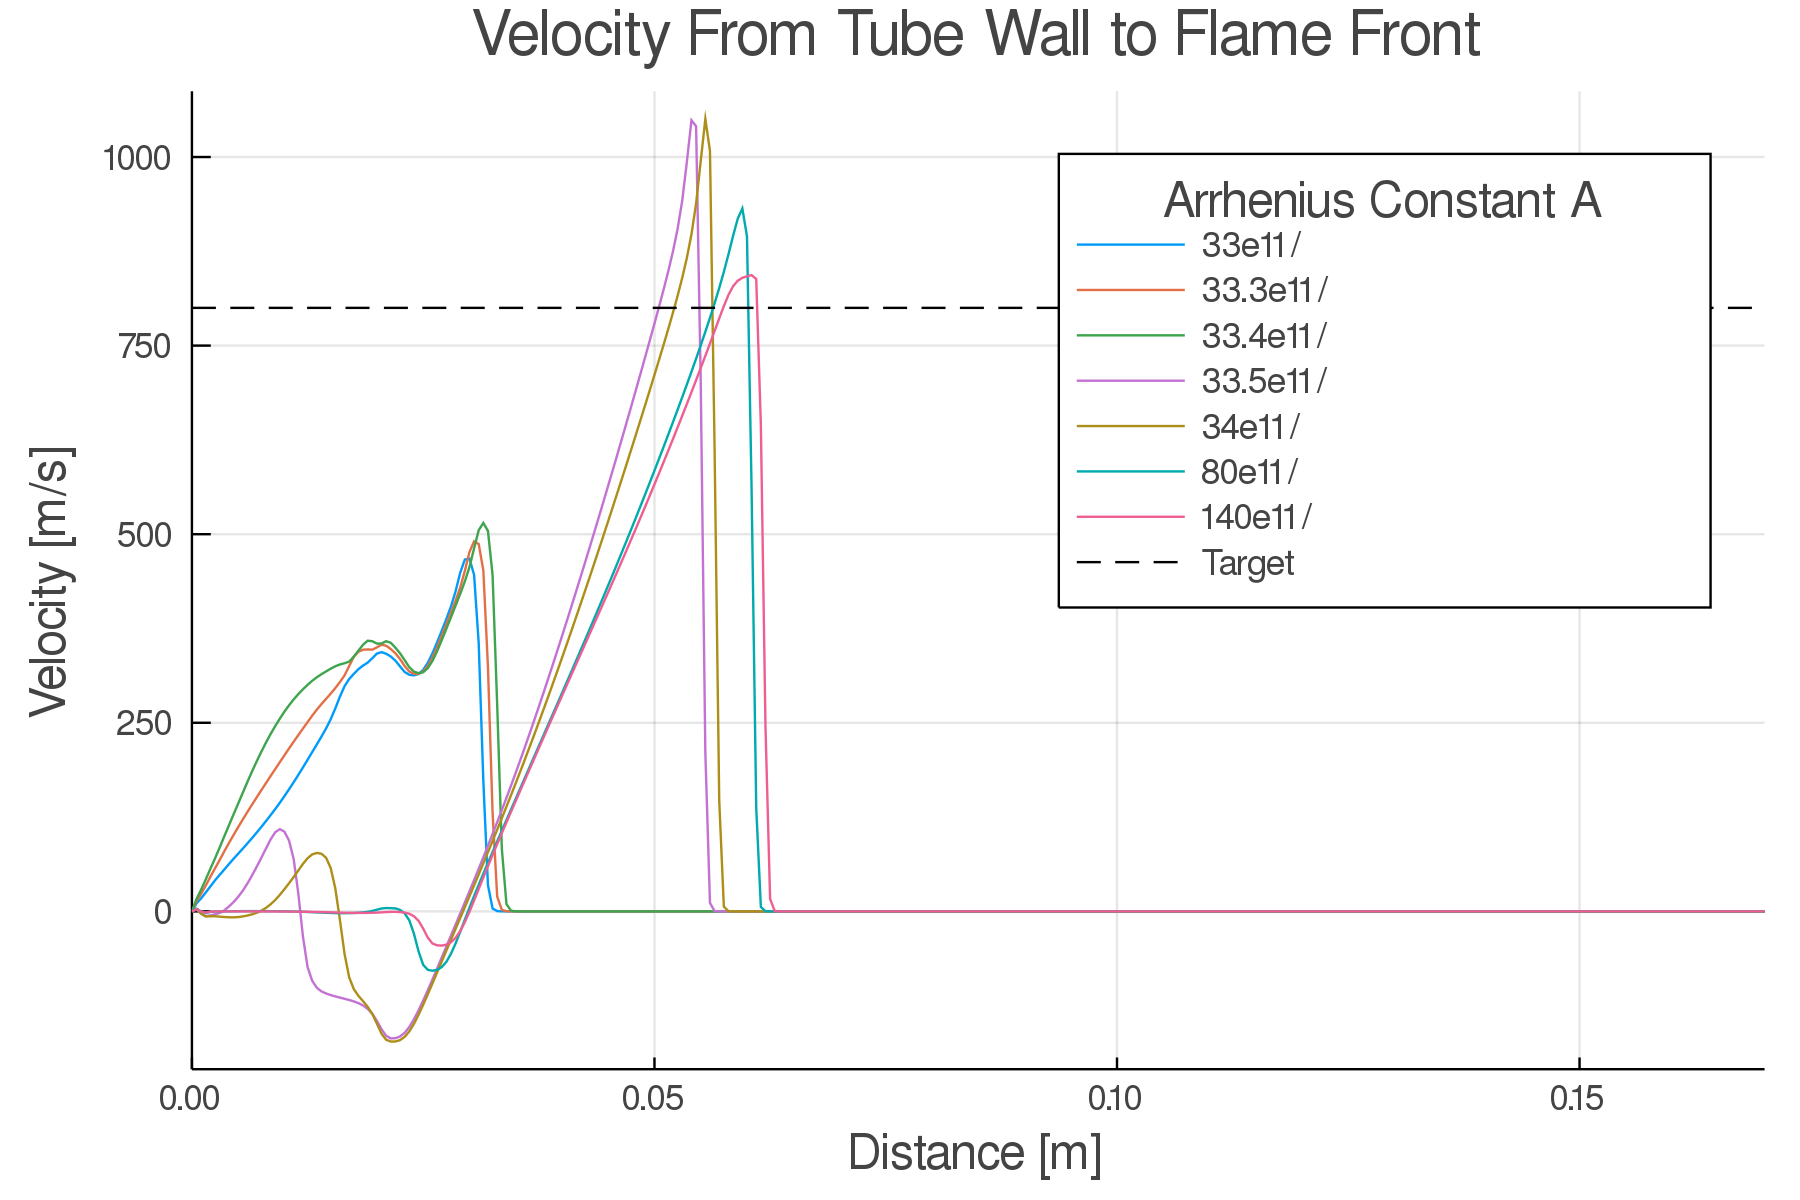
\includegraphics[width=0.8\textwidth]{../figs/example_results/u.png}
\end{center}
\end{frame}